\section{Introduction}

This \cgal\ component implements two surface reconstruction methods which take as input unorganized point sets and compute an implicit function. The output surface mesh is generated by extracting an isosurface of this function with the \cgal\ Surface Mesh Generator~\cite{cgal:ry-gsddrm-06} or potentially with any other surface contouring algorithm. \\

More specifically, the input is an unorganized point set, possibly with attributes such as unoriented or oriented normals. This point set can be analyzed to measure common statistics quantities and bounding volumes such as average spacing, centroid, bounding box and bounding sphere. We can furthermore pre-process the point set before reconstruction with dedicated functions devoted to simplification, outlier removal, smoothing, normal estimation and normal orientation.\\

The core surface reconstruction algorithms consist of computing implicit functions which are either an approximate signed distance function to the inferred surface (Algebraic Point Set Surface - referred to as APSS in the sequel) or an approximate indicator function of the inferred solid (Poisson Surface Reconstruction - referred to as Poisson). Another distinction between the APSS and Poisson algorithms lies into the fact that APSS evaluates the function on the fly at any query point while Poisson requires solving for the implicit function before evaluation. The whole component is structured along a surface reconstruction pipeline.

% Insert image introduction.jpg/eps
\begin{center}
    \label{Surface_reconstruction_3-fig-introduction}
    % Image
    \begin{ccTexOnly}
        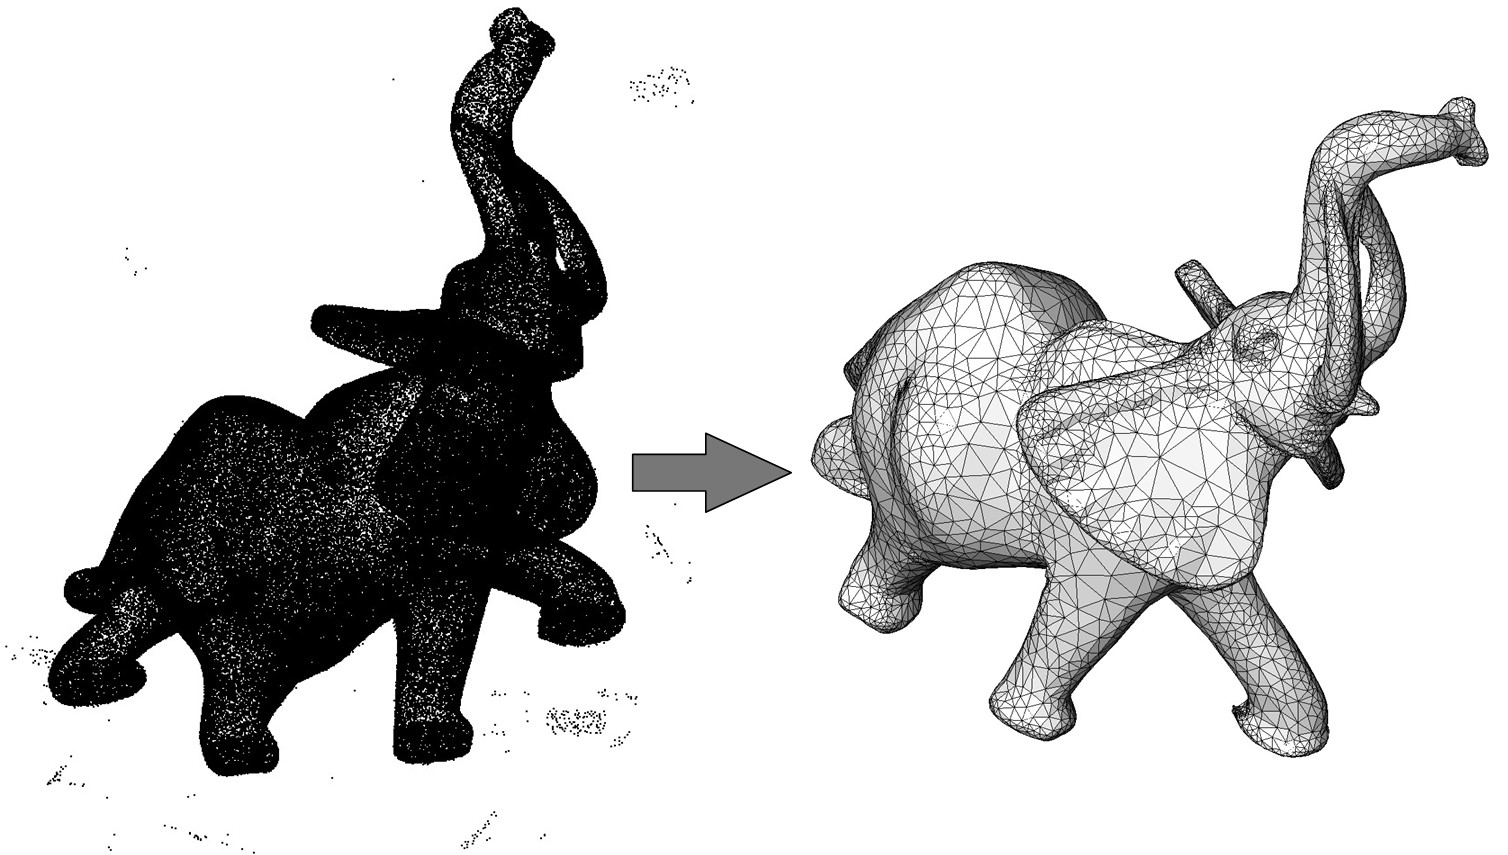
\includegraphics[width=0.9\textwidth]{Surface_reconstruction_3/introduction} % omit .eps suffix
    \end{ccTexOnly}
    \begin{ccHtmlOnly}
        <img width="90%" border=0 src="./introduction.jpg"><P>
    \end{ccHtmlOnly}
    % Title
    \begin{figure}[h]
        \caption{APSS surface reconstruction from 275K
                 points sampled on an elephant
                 with a Minolta laser scanner.}
    \end{figure}
\end{center}


